\documentclass[a4paper, 12pt]{report}
\usepackage[utf8]{inputenc}
\usepackage[boxed,linesnumbered]{algorithm2e}
\usepackage[bookmarks, breaklinks, colorlinks]{hyperref}

\hypersetup{
	citecolor=black,
	linkcolor=black,
	filecolor=black,
	urlcolor=black
}

\usepackage{graphicx}
\usepackage{pdfpages}
\usepackage{tocbibind}
\usepackage{longtable}
\usepackage{array}

\def\chapterautorefname{Chapter}


\title{
	\begin{figure}[h]
		\centering
		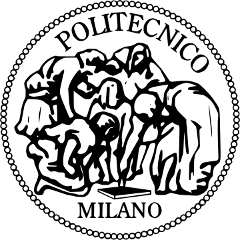
\includegraphics{../common_resources/logo_polimi.png}
	\end{figure}
	\vspace{30px}
	Software Engineering 2 Project: PowerEnJoy \\ \vspace{1em}
	\textbf{I}ntegration \textbf{T}est \textbf{P}lan \textbf{D}ocument
}
	

\author{Marco Ieni, Francesco Lamonaca, Marco Miglionico\\Politecnico di Milano, A.A. 2016/2017}
\date{\today\\v1.0}

\begin{document}
\maketitle
\tableofcontents
% \listoffigures
% \listoftables

\chapter{Introduction}
\label{ch:introduction}
\section{Revision History}
\section{Purpose and Scope}
This document is the Integration Test Plan Document (ITPD) for the PowerEnJoy
software. Its purpose is to determine how to accomplish the
integration test of the software, which tools need to be used and which approach
will be followed.
Integration testing is fundamental activity to guarantee that all the different components of PowerEnjoy interoperate consistently with the requirements they are supposed to fulfil and without unexpected behaviours.
In the following sections we are going to provide:
\begin{itemize}
\item A list of the components and their subcomponents involved in the integration activity that will be tested;
\item The criteria that must be met by the project status before integration testing of the outlined elements may begin;
\item A description of the integration testing approach and the reasoning behind it;
\item The sequence in which the different components will be integrated;
\item A description of the planned testing activities for each integration step, including their input data and the expected output;
\item Some performance measures that should be performed on the components to check that they are fulfilling the requirements;
\item A list of all the tools that will have to be employed during the testing activities, together with a description of the operational environment in which the tests will be executed.
\end{itemize} 

\section{Definitions, acronyms, abbreviations}
\begin{description}
    \item[JPA:] The Java Persistence API (JPA) is a Java application programming interface specification that describes the management of relational data.
    \item[RASD:] Requirements Analysis and Specification Document.
\end{description}

\section{Reference Documents}
This document refers to the project rules of the Software Engineering 2
project, to the template for the Design Document contained into it and to Requirement Analysis and Specification Document (the previous delivered document)


\chapter{Integration Strategy}
\label{ch:integration_strategy}
\section{Entry Criteria}
% Specify the criteria that must be met before integration testing of specific elements may begin (e.g., functions must have been unit tested).
\section{Elements to be Integrated}
In the following paragraph we are going to provide a list of all the components that need to be integrated together.

The integration process of our software is performed on two levels.
\begin{enumerate}
\item \textbf{Low Level:} integration of the different subcomponents (classes, Java Beans) inside the
same subsystem;
\item \textbf{High Level:} integration of different subsystems.
\end{enumerate}

The first step needs to be performed only for the components which contains
the pieces of software that we are going to develop, namely the business
tier, the mobile application in the client tier.
In particular the main subcomponents  that we will integrate are:
\begin{itemize}
\item \textbf{User Manager};
\item \textbf{Email Sender};
\item \textbf{Operator Safe Area Manager};
\item \textbf{User Safe Area Manager};
\item \textbf{Ride Manager};
\item \textbf{Car Manager};
\item \textbf{Fee Manager};
\item \textbf{Payment Manager}
\end{itemize}


The second step need to be performed on the three major high-level components that we outlined in the Design Document,that correspond to the tiers of the system, which – from now on – will
be referred to as subsystems:
\begin{itemize}
\item \textbf{Client tier:} The client tier consists of our mobile application,the operator terminal and the on-board tablet.
\item\textbf{Business tier:} This subsystem implements all the application logic and
communicates with the front-ends.
\item \textbf{Database tier:} This is the DBMS,it is not part of the software to be developed,
but has to be integrated.
\end{itemize}




\section{Integration Testing Strategy}
The integration strategy that we are going to implement is the bottom-up approach. This choice
comes natural since we assume we already have the unit tests for the smallest
components, so we can proceed from the bottom.In this way, we will start integrating together those components that do not depend on other components to operate, or that
only depend on already developed components. The main advantages of this approach are the possibility to perform integration tests on components that are almost fully developed,to obtain feedback on how the system will react and fail in real world situations. The other advantage is that we can start testing the components following the development process,in this way we can reduce time and maximize parallelism.
Moreover, the higher-level subsystems outlined in section 2.2 are well
separated and loosely coupled since they correspond to different tiers. They
also communicate through well-defined interfaces (RESTful API), so
they will not be hard to integrate at a later time.
As we said before the \textbf{Handy Car Board},the \textbf{External System For Driving License Validation}, the \textbf{External System For Payments} and the \textbf{DBMS} are considered as black box, that have already been developed and that can be immediately used in a bottom up approach.


\section{Sequence of Component/Function Integration}

\chapter{Individual Steps and Test Description}
\label{ch:individual_steps}

\chapter{Tools and Test Equipment Required}
\label{ch:tools}

\chapter{Program Stubs and Test Data Required}
\label{ch:program_stubs}

\appendix
\chapter{Appendix}
\section{Used software and tools}
\begin{itemize}
    \item \LaTeX\ \footnote{\url{https://www.latex-project.org/}}, for typesetting this document.
    \item Texmaker\footnote{\url{http://www.xm1math.net/texmaker/}}, for the writing of this document.
    \item GitHub\footnote{\url{https://github.com/}} for version control and distributed work.
    \item Evolus Pencil\footnote{\url{http://pencil.evolus.vn/}} for the mockups.
    \item StarUML\footnote{\url{http://staruml.io/}} for the class diagram.
    \item Alloy Analyzer\footnote{\url{http://alloy.mit.edu/alloy/}} used to build the model generated by the alloy code.
    \item Signavio Academic\footnote{\url{http://academic.signavio.com/p/login}} for the use case diagram and for BPMN.
    \item GitHub desktop\footnote{\url{https://desktop.github.com/}} used to collaborate in the team and to keep track of the changes. 
\end{itemize}

\section{Changelog}

v1.1:
\begin{itemize}
\item added car status flow chart;
\item corrected typos;
\end{itemize}

v1.0:
\begin{itemize}
\item initial release.
\end{itemize}

\section{Work hours}
The statistics about commits and code contribution are available on the GitHub repository of the project\footnote{\url{https://github.com/marcomiglionico94/Software-Engineering-2-Project}}.
Please keep in mind that some commits are the joined effort of two or all the components of the group. However, when this is the case, it is specified in the description of the commit.

These are our estimation of the work hours spent on this project:
\begin{itemize}
    \item Marco Ieni: 38 hours
    \item Francesco Lamonaca: 40 hours
    \item Marco Miglionico: 36 hours
\end{itemize}


\end{document}
